\chapter{\selectlanguage{greek}Προσομοίωση \en{DVB-S2 RA} κώδικα σε κανάλι \en{AWGN}}
Στο κεφάλαιο αυτό, θα παρουσιαστεί ο δέκτης που προσομοιώθηκε και τα αποτελέσματα της προσομοίωσης σε καμπύλες \en{BER} για τους διάφορους ρυθμούς που έχουν προτυποποιηθεί για την ψηφιακή τηλεόραση δεύτερης γενιάς (\en{DVB-S/T2}).

Αρχικά παρουσιάζεται συνοπτικά η διαμόρφωση \en{QPSK} και κατόπιν η διαδικασία αποδιαμόρφωσης (\en{demapping}), μέσω ων έτοιμων συναρτήσεων που παρέχονται από το \en{MATLAB}, καθώς και μέσω ενός \en{A-Posteriori Probability (APP) demapper} που προγραμματίστηκε για το σκοπό αυτό. Στη συνέχεια παρουσιάζεται το σύνολο της προσομοίωσης και στο τέλος του κεφαλαίου, τα αποτελέσματά της.

\section{\en{QPSK Demapper}}
\subsection{Διαμόρφωση \en{QPSK}}
Η κωδική λέξη, μετά την έξοδό της από τον κωδικοποιητή καναλιού, απεικονίζεται στον \en{QPSK} αστερισμό και προκύπτει η ακολουθία μιγαδικών σημάτων, μήκους $n/2$. Σε μορφή ημιτονοειδών κυμάτων μετάδοσης, ο \en{QPSK} αστερισμός γράφεται ως εξής:

\begin{equation}
s_n(t)=\sqrt{\frac{2E_s}{T_s}}\cos\left(2{\pi}f_ct+(2m-1)\frac{\pi}{4}\right),\;\;\;m=1,2,3,4.
\label{eq:QPSK sinusoid waves}
\end{equation}
όπου $E_s$ η ενέργεια συμβόλου, $T_s$ η διάρκεια συμβόλου, $f_c$ η συχνότητα του φέροντος κύματος και $m$ ο δείκτης των συμβώλων. Το αποτέλεσμα είναι ένας δι-διάστατος χώρος σημάτων με μοναδιαίες συναρτήσεις βάσης:

\begin{equation}
\begin{aligned}
\phi_1=\sqrt{\frac{2}{T_s}}\cos(2{\pi}f_ct) \\ \phi_2=\sqrt{\frac{2}{T_s}}\sin(2{\pi}f_ct)
\end{aligned}
\label{eq:QPSK base functions}
\end{equation}
όπου $\phi_1$ είναι η συμφασική και $\phi_2$ η ορθογώνια συνιστώσα. Το σήμα αποτυπώνεται στα 4 σημεία του αστερισμού \en{QPSK} $\left(\pm\sqrt{E_s/2},\pm\sqrt{E_s/2}\right)$ και οι φάσεις των συμβώλων προκύπτουν $\pi/4$, $3\pi/4$, $5\pi/4$ και $7\pi/4$. Ο παραπάνω αστερισμός φαίνεται στο Σχήμα \ref{fig:qpsk constellation}:

\begin{figure}[h]
\center{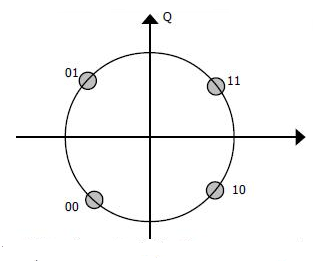
\includegraphics[width=0.55\linewidth]{figures/qpsk_constellation_diagram.png}}
\caption{Ο αστερισμός \en{QPSK}}
\label{fig:qpsk constellation}
\end{figure}
\hfill\\

Στη συνέχεια το σήμα περνάει από το κανάλι μετάδοσης, όπου προστίθεται το \en{AWGN} θόρυβος. Στο δέκτη ακολουθείται η αντίστροφη διαδικασία. Το \en{Matlab} παρέχει έτοιμη μέθοδο αποδιαμόρφωσης και ανίχνευσης μέσω του αντικειμένου \en{comm.QPSKDemodulator} και της μεθόδου \en{step}.

Για την προσομοίωση, προγραμματίστηκε επίσης και ο εξής \en{APP symbol-to-bit demapper}: μετά την έξοδο από το κανάλι η ακολουθία μιγαδικών αριθμών $\mathbf{y}$ μήκους $n/2$ εισάγεται στον \en{demapper}, ο οποίος παράγει μετρικές $L(x_{ij})$ στο διάστημα $(-\infty,\infty)$ για καθένα από τα κωδικά \en{bits} $x_{ij}$, σύμφωνα με τη σχέση:

\begin{equation}
L(x_{ij})=\ln\frac{p(x_{ij}=0\mid\mathbf{y}_i)}{p(x_{ij}=1\mid\mathbf{y}_i)},\;\;\;i\in\left[1,\frac{n}{2}\right],j=1,2.
\label{eq:QPSK LLR}
\end{equation}
οι οποίες εισάγονται στον επαναληπτικό αποκωδικοποιητή για την αρχικοποίησή του.

Από τις εξισώσεις \ref{eq:QPSK sinusoid waves}, \ref{eq:QPSK base functions} προκύπτει πως η διαμόρφωση \en{QPSK} αποτελεί απεικόνιση των δυάδων $\{0,1\}^2$, οι οποίες καλούνται \textit{ετικέτες} (\en{labels}), στο σύνολο των \en{QPSK} σημάτων $S$, δηλαδή $\{0,1\}^2\to{S}$. Αν συμβολιστέι ως ${S}_0^j$  το υποσύνολο των στοιχείων του $S$ που στην \en{j}-οστή θέση της ετικέτας του έχουν 0 και ως ${S}_1^j$ το υποσύνολο των στοιχείων του $S$ που στην \en{j}-οστή θέση της ετικέτας του έχουν 1 και θεωρηθεί απεικόνιση \en{Gray}, προκύπτουν σχηματικά τα υποσύνολα του Σχήματος \ref{fig:qpsk subtotals}.

\begin{figure}[h]
\center{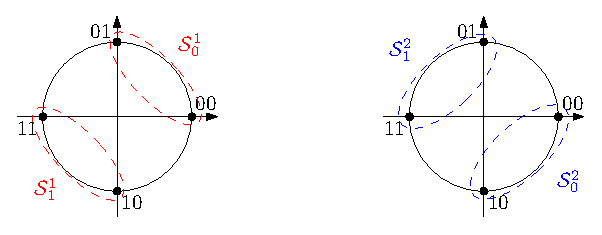
\includegraphics[width=0.55\linewidth]{figures/qpsk.eps}}
\caption{Τα υποσύνολα $ \color{red} {S}_1^0$, $ \color{red} {S}_1^1$ και $ \color{blue} {S}_0^0$, $ \color{blue}{S}_0^1$}
\label{fig:qpsk subtotals}
\end{figure}

Η σχέση \ref{eq:QPSK LLR} μπορεί να αναλυθεί περεταίρω για το κωδικό \en{bit} $L(x_{i1})$, αν εφαρμοστεί ο νόμος ολικής πιθανότητας, επιμερίζοντας σε όλα τα γεγονότα $x_{i2}$, το γεγονός $\{x_{i1}=0\}$ στον αριθμητή και το $\{x_{i1}=1\}$ στον παρονομαστή, ώστε να πάρει την μορφή της εξίσωσης \ref{eq:fraction 4.1}:

\begin{equation}
\begin{split}
L(x_{i1}) & =\ln\frac{\sum\nolimits_{x_{i2}}p(x_{i1}=0, x_{i2}\mid\mathbf{y}_i)}{\sum\nolimits_{x_{i2}}p(x_{i1}=1, x_{i2}\mid\mathbf{y}_i)} \\
& = \ln\frac{\sum\nolimits_{\mathbf{s}\in{S}_0^1} p(\mathbf{s}\mid\mathbf{y}_i)}{\sum\nolimits_{\mathbf{s}\in{S}_1^1} p(\mathbf{s}\mid\mathbf{y}_i)}
\end{split}
\label{eq:fraction 4.1}
\end{equation}

Γενικεύοντας από την εξίσωση \ref{eq:fraction 4.1}, για το κωδικό \en{bit} $L(x_{ij})$, προκύπτει:

\begin{equation}
\begin{split}
L(x_{ij}) & = \ln\frac{\sum\nolimits_{\mathbf{s}\in{S}_0^j} p(\mathbf{s}\mid\mathbf{y}_i)}{\sum\nolimits_{\mathbf{s}\in{S}_1^j} p(\mathbf{s}\mid\mathbf{y}_i)} \\
& = \ln\frac{\sum\nolimits_{\mathbf{s}\in{S}_0^j} p(\mathbf{y}_i\mid\mathbf{s})p(\mathbf{s})}{\sum\nolimits_{\mathbf{s}\in{S}_1^j} p(\mathbf{y}_i\mid\mathbf{s})p(\mathbf{s})} \\
& = \ln\frac{\sum\nolimits_{\mathbf{s}\in{S}_0^j} p(\mathbf{y}_i\mid\mathbf{s})}{\sum\nolimits_{\mathbf{s}\in{S}_1^j} p(\mathbf{y}_i\mid\mathbf{s})}
\end{split}
\label{eq:fraction 4.2}
\end{equation}

Οι ισότητες λογαρίθμων στην εξίσωση \ref{eq:fraction 4.2} προκύπτουν χρησιμοποιώντας τον κανόνα του \en{Bayes} και υποθέτοντας ότι τα σήματα $\mathbf{s} \in S$ είναι ισοπίθανα.

Ακόμη για το διακριτό κανάλι \en{AWGN}, η κατανομή πυκνότητας πιθανόητας $p(\mathbf{y}_i\mid\mathbf{s})$ ορίζεται ως εξής:

\begin{equation}
p(\mathbf{y}_i\mid\mathbf{s})=\frac{1}{2\pi\sigma^2}\exp\left\{-\frac{{\norm{\mathbf{y}_i-\mathbf{s}}}^{2}}{2\sigma^2}\right\}
\label{eq:AWGN pdf}
\end{equation}

Συνοψίζοντας, η εξίσωση \ref{eq:fraction 4.1}, λόγω των \ref{eq:fraction 4.2}, \ref{eq:AWGN pdf} γίνεται:

\begin{equation}
\begin{split}
L(x_{ij}) & =\ln \frac{\sum \nolimits_{\mathbf{s}\in{S}_0^j} \exp \left\{ -\frac{\norm{\mathbf{y}_i}^2 -2\Re(\mathbf{y}_i\cdot\mathbf{s}) + \norm{\mathbf{s}}^2}{2\sigma^2} \right\}}{\sum \nolimits_{\mathbf{s}\in{S}_1^j} \exp \left\{ -\frac{\norm{\mathbf{y}_i}^2 -2\Re(\mathbf{y}_i\cdot\mathbf{s}) + \norm{\mathbf{s}}^2}{2\sigma^2} \right\}} \\
& =\ln \frac{\sum \nolimits_{\mathbf{s}\in{S}_0^j} \exp \left\{ \frac{\Re(\mathbf{y}_i\cdot\mathbf{s})}{\sigma^2}\right\}}{\sum \nolimits_{\mathbf{s}\in{S}_1^j} \exp \left\{ \frac{\Re(\mathbf{y}_i\cdot\mathbf{s})}{\sigma^2}\right\}}
\end{split}
\label{eq:fraction 4.3}
\end{equation}

Στην εξίσωση \ref{eq:fraction 4.3}, θεωρώντας πως η ενέργεια σήματος $\norm{\mathbf{s}}^2=E_s,\;\forall \; \mathbf{s} \in S$ είναι η ίδια, οι παράγοντες $\exp\left\{-\frac{\norm{\mathbf{y}_i}^2}{2\sigma^2}\right\}$, $\exp\left\{-\frac{\norm{\mathbf{s}}^2}{2\sigma^2}\right\}$ μπορούν να απαλειφθούν με παραγοντοποίηση σε αριθμητή και παρονομαστή και τελικά η εξίσωση \ref{eq:fraction 4.3} να λάβει τη μορφή:

\begin{equation}
L(x_{ij})=\ln\frac{\sum \nolimits_{\mathbf{s}\in{S}_0^j}\exp\left\{\frac{y_{iI}s_I+y_{iQ}s_Q}{\sigma^2}\right\}}{\sum \nolimits_{\mathbf{s}\in{S}_1^j}\exp\left\{\frac{y_{iI}s_I+y_{iQ}s_Q}{\sigma^2}\right\}}
\label{eq:fraction 4.4}
\end{equation}
όπου οι δείκτες $I$, $Q$ υποδεικνύουν προβολή του αντίστοιχου διανύσματος στη συμφασική και στην ορθογώνια συνιστώσα αντίστοιχα.

\section{Προσομοίωση στο \en{Matlab}}
% \selectlanguage{english}
% \lstinputlisting{spa9.m}
% \selectlanguage{greek}
\begin{table}[h]
\centering
\begin{tabular}
{>{\bfseries}c*{2}{c}}\toprule\toprule{\en{Rate R}} & {$(E_b/N_0)_{soft}\;\;(dB)$}\\ \midrule
1/4&-0.793\\
1/3&-0.497\\
2/5&-0.236\\
1/2&0.187\\
3/5&0.682\\
2/3&1.059\\
3/4&1.626\\
4/5&2.039\\
9/10&3.199\\ \bottomrule\bottomrule
\end{tabular}
\caption{Χωρητικότητα ως \en{$E_b/N_0$} για τους ρυθμούς κώδικα της προσομοίωσης}
\label{table: EbN0 limits}
\end{table}

Στον πίνακα \ref{table: EbN0 limits}, φαίνεται το (θεωρητικό) κάτω όριο $E_b/N_0$ για τον κάθε ρυθμό κώδικα που προσομοιώνεται, το οποίο καλείται \textit{όριο κωδικοποίησης} και αντιστοιχεί σε διαμόρφωση \en{BPSK} ή \en{QPSK}. Η χωρητικότητα, όπως εκφράζεται από τα παραπάνω όρια για δεδομένο ρυθμό \en{R}, δίνει ένα κατώφλι \en{SNR} μετά από το οποίο και με τη χρήση κωδικοποίησης καναλιού, μπορεί να επιτευχθεί -θεωρητικά- αξιόπιστη επικοινωνία, σε διαφορετική περίπτωση η αξιοπιστία της οποίας είναι μη ελέγξιμη.

\section{Αποτελέσματα}
Σε αυτή την ενότητα παρουσιάζονται τα αποτελέσματα. Ταυτόχρονα με τη συγγραφή του Κεφαλαίου 3, θα ανανεώνεται και αυτή η παράγραφος με διαγράμματα.